% ------------------------------------------------------------------------------
% Resultados
% ------------------------------------------------------------------------------

\chapter{Resultados}
\label{chap_resultados}

Este capitulo apresenta os resultados obtidos nas cinco etapas da pratica, com base nas simulacoes registradas em arquivos CSV e nas figuras geradas automaticamente. Consideraram-se duas escalas amostrais: 10 caminhadas na analise principal de trajetorias e 50000 caminhadas independentes na etapa de verificacao do TCL.

\section{Trajetórias das 10 Caminhadas (\texorpdfstring{$N=10000$}{N=10000})}

A Figura~\ref{fig:caminhadas_10} apresenta as 10 trajetorias simuladas com 10000 passos. Como esperado para um processo sem vies, observa-se alternancia entre periodos de crescimento e decrescimento, com flutuacoes de amplitude crescente ao longo do tempo.

\begin{figure}[H]
	\centering
	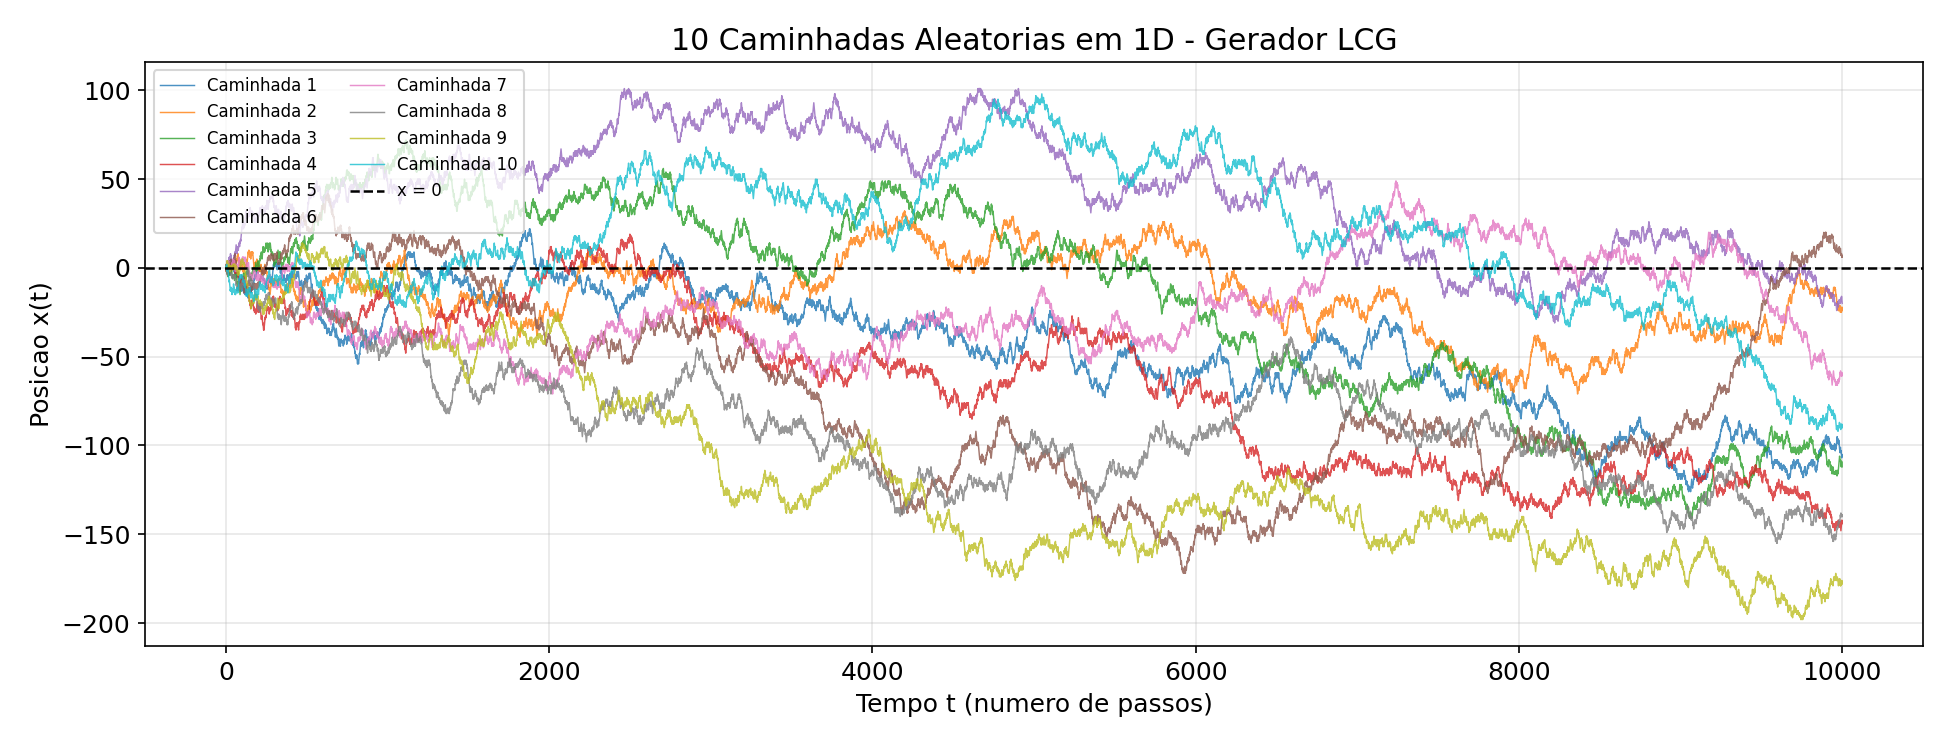
\includegraphics[width=0.95\textwidth]{figuras/graficos/caminhadas.png}
	\caption{Dez trajetorias de random walk 1D com 10000 passos cada.}
	\label{fig:caminhadas_10}
\end{figure}

Os deslocamentos finais observados em $t=10000$ foram:
\begin{equation}
(-106, -24, -112, -144, -20, 6, -60, -140, -178, -90).
\end{equation}

A media amostral desses deslocamentos foi $\bar{x}_{\text{final}}=-86{,}8$, indicando que, para apenas 10 realizacoes, ainda pode ocorrer assimetria amostral relevante, mesmo em um processo teoricamente centrado em zero.

\section{Desvio Quadrático Médio e Ajuste Log-Log}

A Figura~\ref{fig:msd_loglog} mostra o comportamento de $\langle R^2(t)\rangle$ e o ajuste por lei de potencia.

\begin{figure}[H]
	\centering
	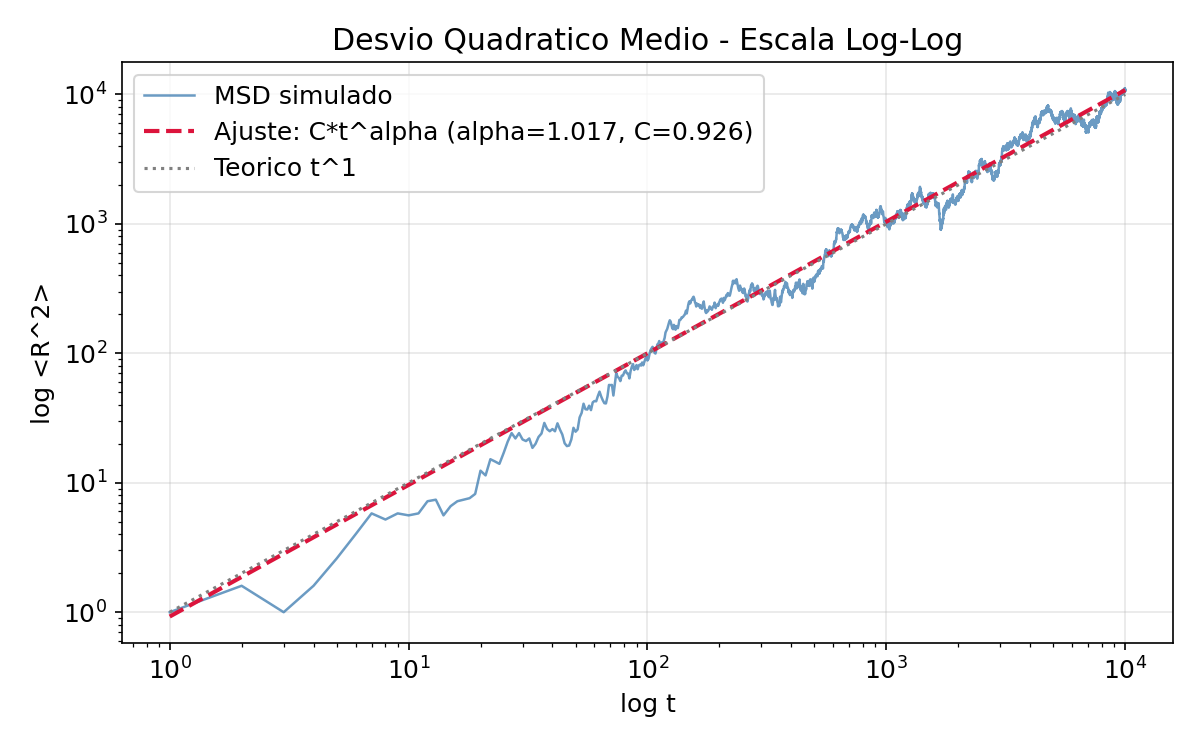
\includegraphics[width=0.85\textwidth]{figuras/graficos/msd_loglog.png}
	\caption{Ajuste de lei de potencia para o desvio quadratico medio em escala log-log.}
	\label{fig:msd_loglog}
\end{figure}

Os parametros estimados foram:
\begin{equation}
\hat{\alpha}=1{,}0168, \qquad \hat{C}=0{,}9261,
\end{equation}
com coeficiente de determinacao $R^2=0{,}9608$. O valor de $\hat{\alpha}$, proximo de 1, indica comportamento compativel com o crescimento aproximadamente linear esperado para random walk classico.

\section{Teste de Hipótese para o Expoente}

Para o teste bilateral previsto no item 4 do roteiro, considerou-se:
\begin{equation}
H_0: \alpha = 1
\quad \text{versus} \quad
H_1: \alpha \neq 1.
\end{equation}

Os valores obtidos no ajuste e no teste foram:
\begin{itemize}
    \item $\hat{\alpha}=1{,}016797$ e $\mathrm{SE}(\hat{\alpha})=0{,}002053$;
    \item $t=8{,}180660$ com $gl=9998$;
    \item $t_{\mathrm{crit}}=1{,}960201$ (nivel de 5\%, bilateral);
    \item $p\text{-valor}=3{,}17\times10^{-16}$.
\end{itemize}

\begin{equation}
\text{Decisao}(\alpha=5\%) =
\begin{cases}
\text{rejeitar } H_0, & \text{se } |t| > t_{\mathrm{crit}} \; \text{(ou } p\text{-valor} < 0{,}05\text{)}, \\
\text{nao rejeitar } H_0, & \text{caso contrario}.
\end{cases}
\end{equation}

Aplicando a regra acima, tem-se \(|t| > t_{\mathrm{crit}}\) e \(p\text{-valor} < 0{,}05\); portanto, \textbf{rejeita-se} $H_0$ no sentido estritamente estatistico. Um intervalo de confianca aproximado de 95\% para $\alpha$ e $[1{,}0128,\,1{,}0208]$, que nao contem 1.

Essa conclusao estatistica nao invalida a interpretacao fisica geral de processo difusivo: com grande numero de pontos no ajuste, desvios pequenos de $\alpha$ em relacao a 1 tendem a se tornar estatisticamente detectaveis. Desse modo, o resultado pode ser interpretado como evidencia de leve desvio do valor ideal em um experimento numerico finito, mantendo comportamento global proximo ao random walk classico.

\section{Verificação do Teorema Central do Limite}

Na etapa de TCL, os passos por caminhada foram mantidos iguais ao experimento principal ($N_{\text{steps,TCL}}=N_{\text{steps}}=10000$) e foi aumentado apenas o numero de caminhadas independentes para 50000. Assim, analisa-se a variavel normalizada $Z=S_N/\sqrt{N}$ com amostra maior, sem alterar a escala temporal de cada caminhada. A Figura~\ref{fig:tcl_hist} apresenta o histograma de $Z$ comparado a curva normal de referencia.

\begin{figure}[H]
	\centering
	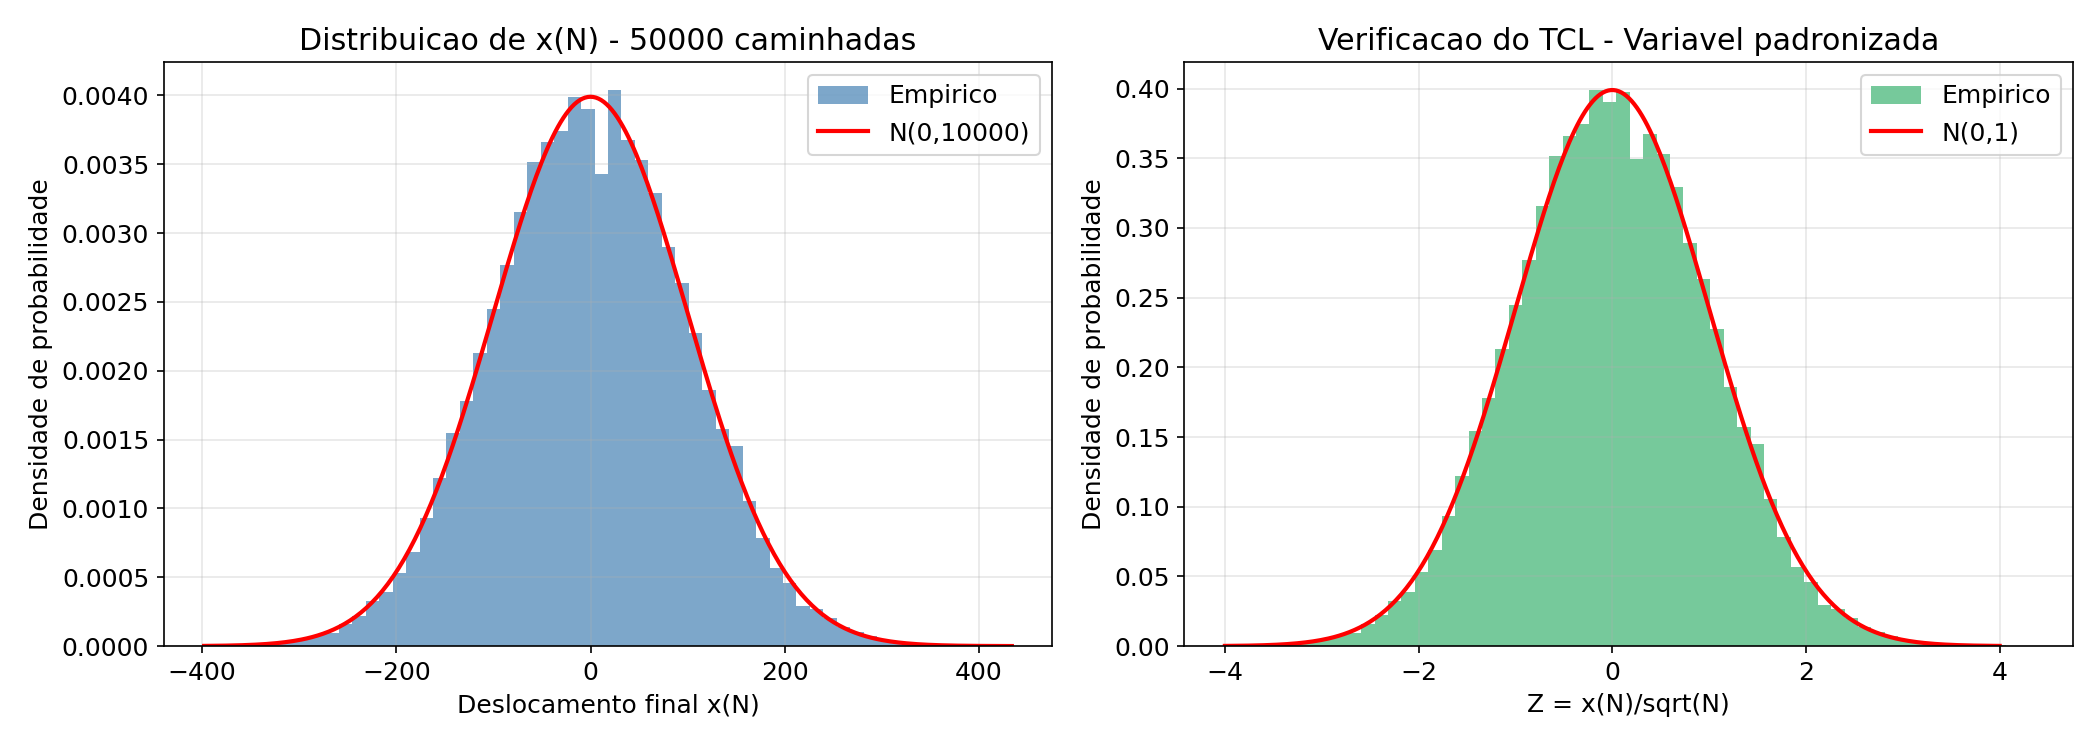
\includegraphics[width=0.85\textwidth]{figuras/graficos/tcl.png}
	\caption{Histograma da variavel normalizada $Z$ e comparacao com distribuicao normal padrao.}
	\label{fig:tcl_hist}
\end{figure}

As metricas obtidas foram: media $\bar{Z}\approx 8,0\times10^{-5}$, desvio padrao $\sigma_Z\approx 0,9863$, estatistica Kolmogorov-Smirnov $D=0,0127$ e $p$-valor $=0,3895$. Como o $p$-valor e superior a 0,05, nao ha evidencia para rejeitar a compatibilidade com normalidade, reforcando a aderencia ao TCL. A formulacao do teste K-S utilizada segue a definicao padrao para adequacao de distribuicao \cite{nist_ks_test}.

\section{Síntese dos Resultados}

Em conjunto, os resultados indicam que: (i) a implementacao do LCG gerou trajetorias plausiveis para random walk simples; (ii) o crescimento de $\langle R^2(t)\rangle$ permaneceu muito proximo de linear; e (iii) os deslocamentos finais normalizados apresentaram comportamento gaussiano consistente com o limite central.



